\section{Part C}
What is the statistic you would compute to test this hypothesis and its theoretical distribution?\\
-----\\

I'm going to reasonably assume the measurement of US car mileages have no dependency on Japanese car mileages and vice versa. That being said, the hypothesis in part B is a statement on the comparison of average mileage, which I framed in that manner because the claim from the problem context comments on what people usually claim about these cars, so a comparison of average mileage of these cars ought to be most appropriate.\\

With that established, choosing an appropriate test to compare the means of two independent groups immediately brings two-sample Student's t-test to mind. This test requires that the groups be independent, that the samples should be about Normal, and their variances should be about the same. Below is the function and corresponding Q-Q Plot I generated to see how closely each group resembles a Gaussian:

\begin{verbatim}
def main():
    data = pd.read_csv('../datasets/cars.csv', header=None)
    us_mileage = data[0].dropna().to_numpy()
    jp_mileage = data[1].dropna().to_numpy()

    sns.set_style("whitegrid")
    sns.set_palette("muted")
    _, axes = plt.subplots(1, 2, figsize=(12, 6))

    percentiles = np.linspace(0, 100, 75)
    norm_quantiles_us = np.percentile(np.random.normal(loc=np.mean(us_mileage), 
    scale=np.std(us_mileage), size=10_000), percentiles)
    sample_quantiles_us = np.percentile(us_mileage, percentiles)

    norm_quantiles_jp = np.percentile(np.random.normal(loc=np.mean(jp_mileage), 
    scale=np.std(jp_mileage), size=10_000), percentiles)
    sample_quantiles_jp = np.percentile(jp_mileage, percentiles)

    axes[0].scatter(norm_quantiles_us, sample_quantiles_us, alpha=0.5, 
                    s=20, color='blue', edgecolor='blue')
    axes[0].plot([min(norm_quantiles_us), max(norm_quantiles_us)],
                 [min(norm_quantiles_us), max(norm_quantiles_us)],
                 'k--', lw=2, alpha=0.7)
    axes[0].set_title("Q-Q Plot: US Cars Mileage", fontsize=14)
    axes[0].set_xlabel("Theoretical Quantiles", fontsize=12)
    axes[0].set_ylabel("Sample Quantiles", fontsize=12)

    axes[1].scatter(norm_quantiles_jp, sample_quantiles_jp, alpha=0.5, 
                    s=20, color='purple', edgecolor='purple')
    axes[1].plot([min(norm_quantiles_jp), max(norm_quantiles_jp)],
                 [min(norm_quantiles_jp), max(norm_quantiles_jp)],
                 'k--', lw=2, alpha=0.7)
    axes[1].set_title("Q-Q Plot: Japanese Cars Mileage", fontsize=14)
    axes[1].set_xlabel("Theoretical Quantiles", fontsize=12)
    axes[1].set_ylabel("Sample Quantiles", fontsize=12)

    plt.tight_layout()
    plt.savefig(f"../figures/qqplot.png", bbox_inches='tight', dpi=300)
\end{verbatim}

\begin{center}
    \textbf{Figure 2:} Function for plotting theoretical against sample quantiles for US and Japanese cars.\\
\end{center}

\begin{center}
    
\includegraphics[width=0.95\textwidth]{figures/qqplot.png}
    \textbf{Figure 3:} Q-Q plots for US and Japanese cars quantiles.\\
\end{center}

The quantiles for both the US cars and the Japanese cars stay close to the agreement line through the Q-Q Plot, especially toward the middle quantiles, though they do both have a couple that visually deviate quite far from the agreement line in the more extreme cases. The plot seems to suggest they are both approximately Normal, but it would be helpful to also visualize the distribution shape directly as well, not to mention they could be plotted on the same figure to give a general idea of which country may be produce higher mileage cars in the average-case:

\begin{verbatim}
def main():
    data = pd.read_csv('../datasets/cars.csv', header=None)
    us_mileage = data[0].dropna()
    jp_mileage = data[1].dropna()

    sns.set_style("whitegrid")
    sns.set_palette("muted")

    plt.figure(figsize=(10, 6))

    sns.histplot(us_mileage, bins=30, kde=False, color='blue', edgecolor='white', 
    alpha=0.6, label='US Cars')
    sns.histplot(jp_mileage, bins=30, kde=False, color='red', edgecolor='white', 
    alpha=0.6, label='Japanese Cars')

    plt.title('Histogram: US vs Japanese Cars Mileage', fontsize=16)
    plt.xlabel('Mileage', fontsize=14)
    plt.ylabel('Count', fontsize=14)
    plt.legend(fontsize=12)

    plt.tight_layout()
    os.makedirs("../figures", exist_ok=True)
    plt.savefig("../figures/histogram.png", bbox_inches='tight', dpi=300)
\end{verbatim}

\begin{center}
    \textbf{Figure 4:} Function for plotting US and Japanese car mileage distributions.\\
\end{center}

\begin{center}
    
\includegraphics[width=0.95\textwidth]{figures/histogram.png}
    \textbf{Figure 5:} Histogram plots for US and Japanese cars mileages.\\
\end{center}

This result gives us pretty decent visual confirmation that these groups both approximate Normal distributions, and the addition histogram plot does well to visualize the peculiarities in the distribution mass that attribute to the deviations from the agreement line that we saw in the Q-Q Plot. For example, the heavier left tail of the US car distribution corresponding to the deviations above the agreement line or the right tail tapering off a bit faster than the right in the case of Japanese car mileages corresponding to the deviations below the agreement line. Also like I mentioned, the histogram gives us a rough confirmation that the average Japanese car mileage is higher than the US cars.\\

We need to also confirm that the variance are about the same, so for this purpose I produced box plots corresponding to each country:

\begin{verbatim}
def main():
    data = pd.read_csv('../datasets/cars.csv', header=None)
    us_mileage = data[0].dropna()
    jp_mileage = data[1].dropna()

    df = pd.DataFrame({
        'Mileage': pd.concat([us_mileage, jp_mileage], ignore_index=True),
        'Region': ['US'] * len(us_mileage) + ['Japan'] * len(jp_mileage)
    })

    sns.set_style("whitegrid")
    sns.set_palette("muted")

    plt.figure(figsize=(8, 6))
    ax = sns.boxplot(x='Region', y='Mileage', data=df, showfliers=True)

    ax.set_title('Car Mileages for US vs Japanese Cars', fontsize=16)
    ax.set_xlabel('')
    ax.set_ylabel('Mileage', fontsize=12)

    plt.tight_layout()
    plt.savefig("../figures/boxplot.png", bbox_inches='tight', dpi=300)
\end{verbatim}

\begin{center}
    \textbf{Figure 6:} Function for plotting US and Japanese car mileages as box plots.\\
\end{center}

\begin{center}
    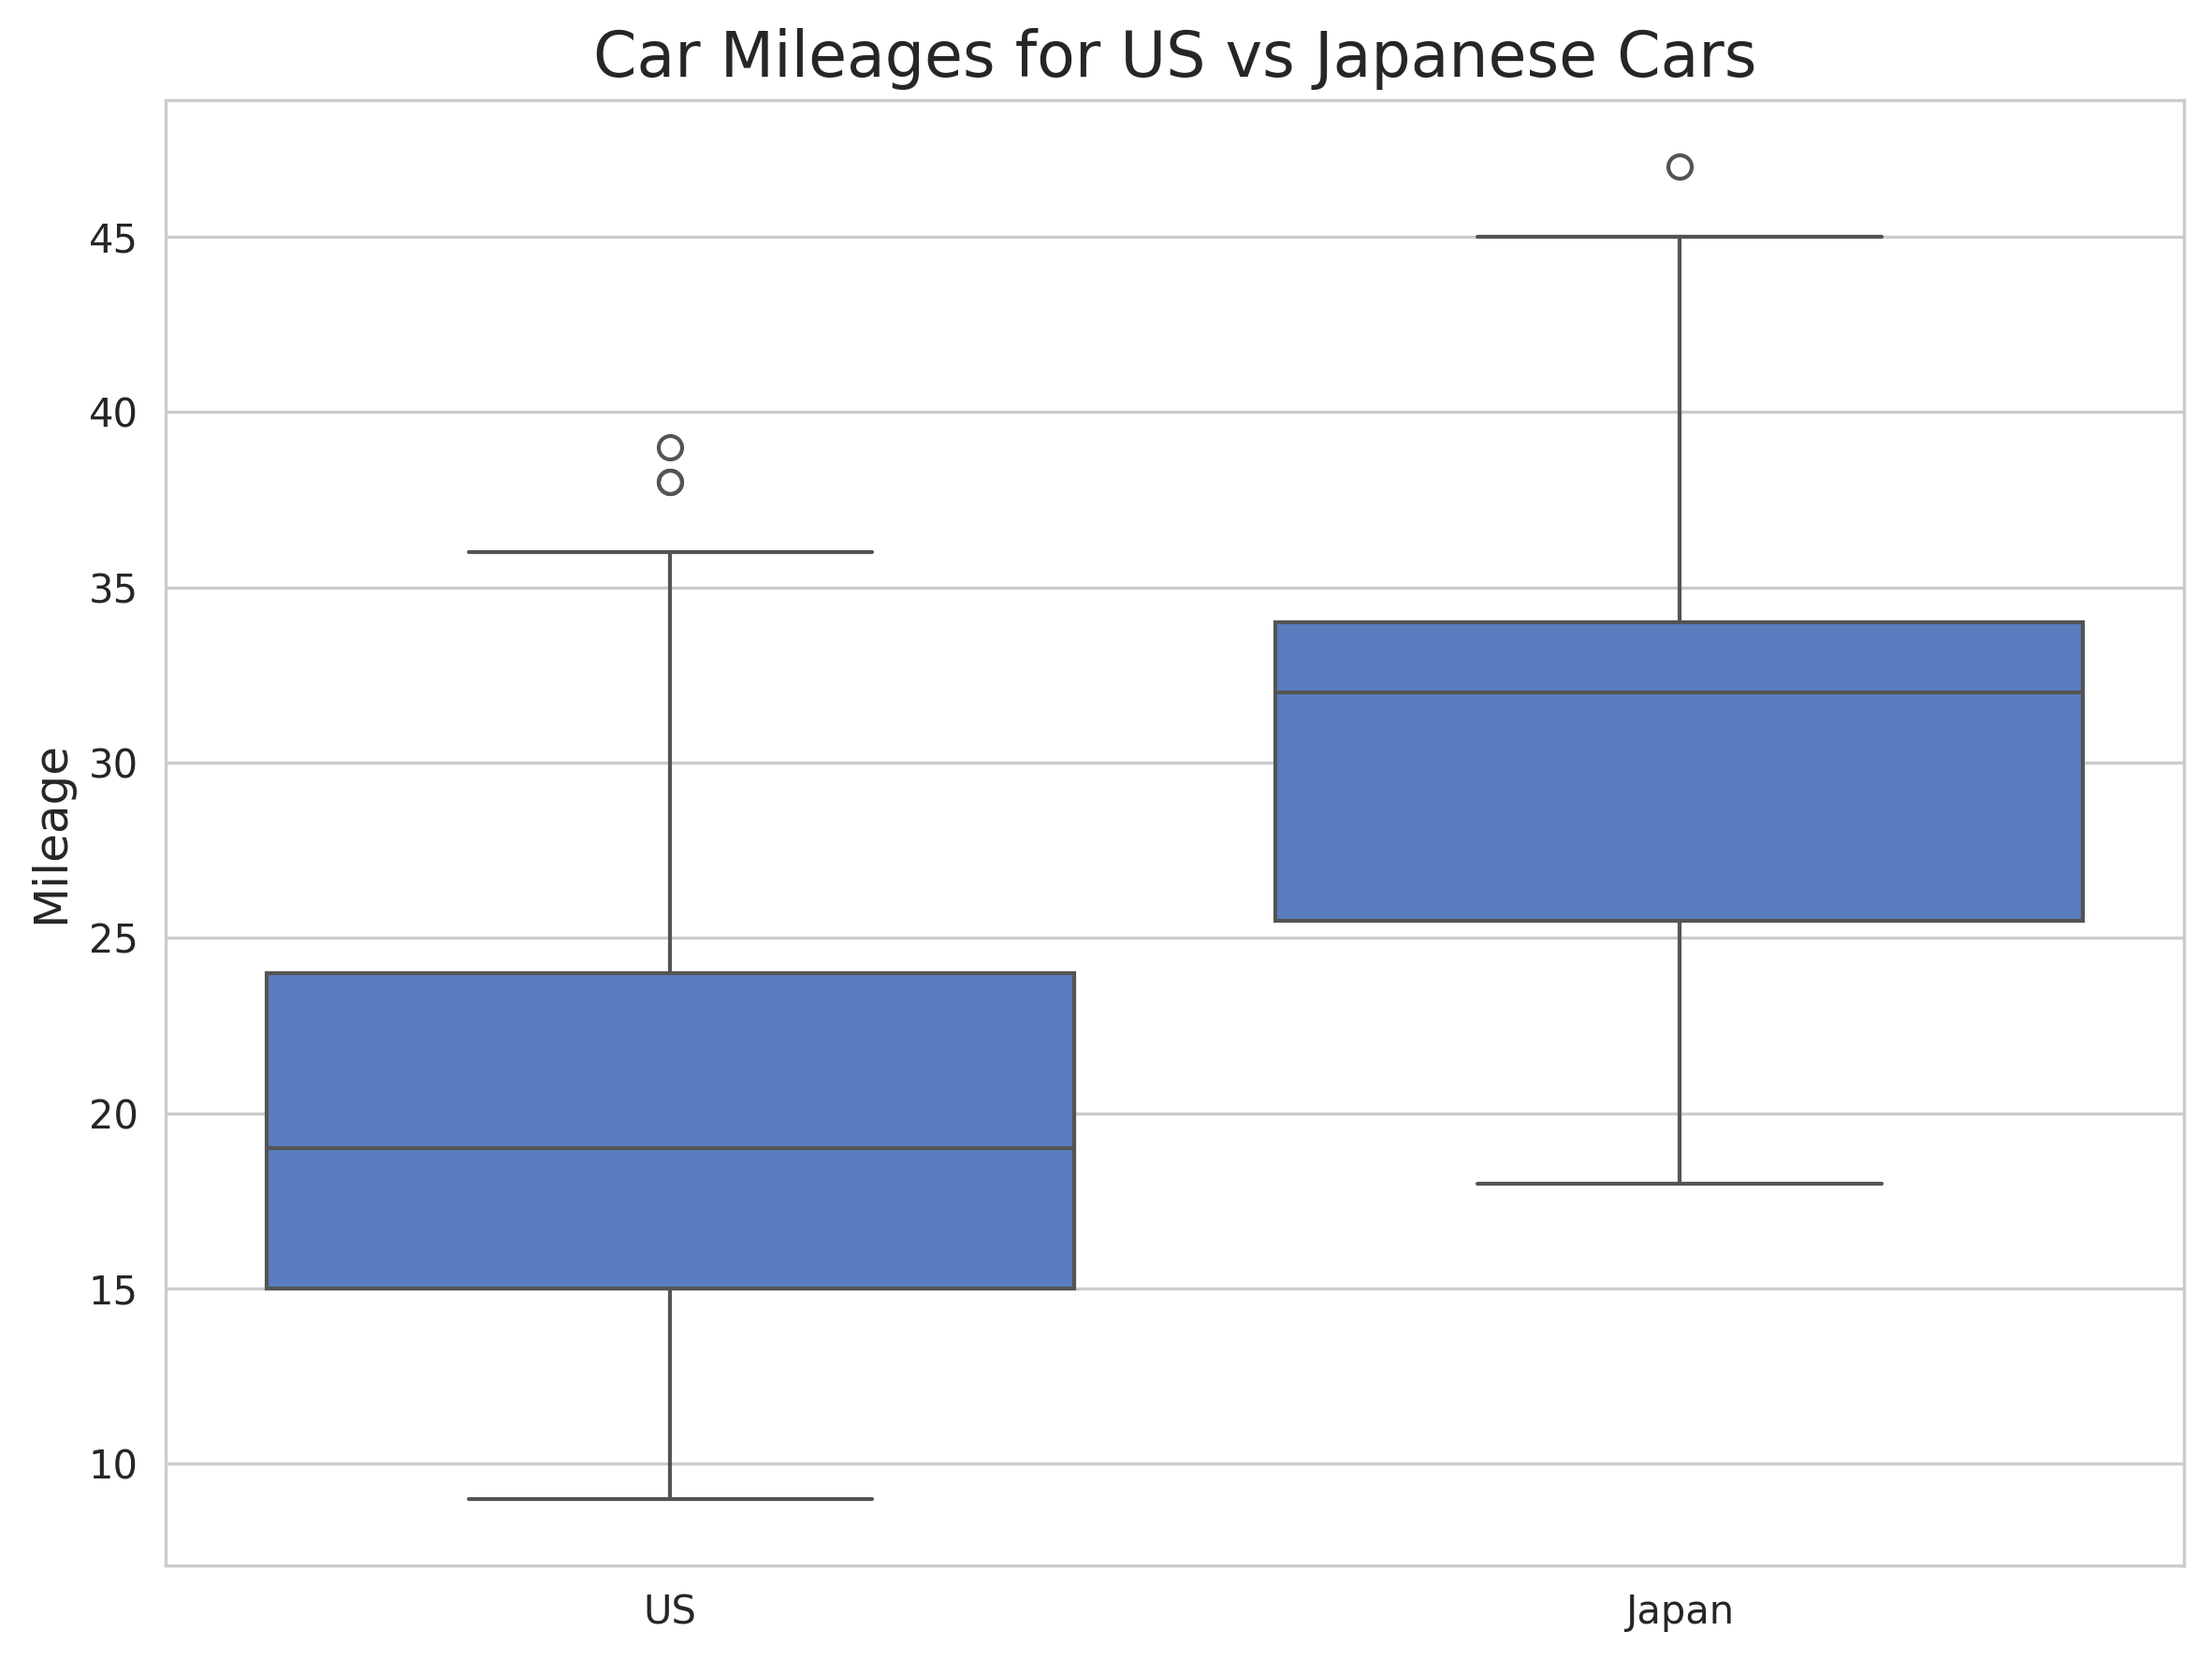
\includegraphics[width=0.95\textwidth]{figures/boxplot.png}
    \textbf{Figure 7:} Box plots for US and Japanese cars mileages.\\
\end{center}

The box plots show a very promising signal that their inter-quartile ranges are about the same size and it shows that their whiskers protrude by about the same amount both above and below their IQR. We can also see a comparison of the medians from this visual, and given that the respective distributions are sufficiently symmetrical, then we have another rough signal that the Japanese cars may greater mileage on average.\\

That being said, these visualizations confirm that the underlying conditions of the t-test have been adequately met. This test statistic follows a t-distribution, which models the sampling distribution of the standardized difference between sample means. It is similar to the Normal distribution but with heavier tails, especially for smaller sample sizes, reflecting an increased uncertainty. In this case, the t-distribution can be expressed as:\\

$$
t = \frac{\bar{x}_{\text{jp}} - \bar{x}_{\text{us}}}{\sigma_{\bar{x}_{\text{jp}} - \bar{x}_{\text{us}}}}
$$

where $\sigma_{\bar{x}_\text{jp} - \bar{x}_\text{us}}$ is the standard error of the difference between sample means:

$$
\sigma_{\bar{x}_{\text{jp}} - \bar{x}_{\text{us}}} = \sqrt{\frac{\sigma_{\text{jp}}^2}{n_{\text{jp}}} + \frac{\sigma_{\text{us}}^2}{n_{\text{us}}}}
$$

This test statistic follows this distribution with $ n_{\text{jp}} + n_{\text{us}} - 2 $ degrees of freedom under $ H_0 $. Because $ H_1 $ is one-sided (Japanese > US), I will perform a right-tailed test, rejecting $ H_0 $ if the t-statistic is sufficiently large.

\newpage
